\documentclass[12pt, a4paper]{ctexart}
\usepackage{graphicx, natbib}
\usepackage{indentfirst, amsmath}
\usepackage{tikz}
%\usepackage{fancyhdr}
%\fancyhf{}
%\pagestyle{fancy}
%\fancypagestyle{fancy}{%
%	\fancyhf{}%
%	\fancyhead[C]{\fangsong 材料力学课程研究报告}
%	\fancyfoot[C]{\thepage}%
%	\renewcommand{\headrulewidth}{0pt}
%}
\usepackage{fancyhdr}
\pagestyle{fancy}
\lhead{}
\rhead{}
\chead{\fangsong 材料力学课程研究报告} 
\cfoot{}
\rfoot{\thepage} 
\renewcommand{\headrulewidth}{0.4pt} 
\renewcommand{\footrulewidth}{0pt}

\title{任意三维应力状态下的正应力}
\begin{document}
%%%%%%%%%%%%%%%%%%%%%%%%%%%%%%
%% 封面部分
%%%%%%%%%%%%%%%%%%%%%%%%%%%%%%
\begin{titlepage}
	\centering
%	
\includegraphics[width=0.2\textwidth]{./templetes/image.png}\par
%	\vspace{1cm}
	
\includegraphics[width=1.0\textwidth]{./templates/logo.png}\par
%	\vspace{0.1cm}
%	
\includegraphics[width=0.8\textwidth]{./templetes/title_e.png} \par
	\vspace{2cm}
	{\kaishu\LARGE 材料力学课程研究报告\par}
	\vspace{1.5cm}
	{\fontsize{30pt}{\baselineskip}\heiti 任意三维应力状态下的正应力\par}
	\vspace{2cm}
	{\fangsong\Large\itshape 吴思源\par}
	\vfill
	{2171310846}\par
	\fangsong{自动化钱71}

	\vfill
% Bottom of the page
	{\large \today\par}
\end{titlepage}

\maketitle
\section{牵引向量和应力分量}
为方便描述复杂应力情形下单元体的应力状态,先建立具有基矢量的笛卡尔坐标系,并使基矢量之一是表面的法线,并且坐标系的原点位于牵引作用的点,如图\ref{fig1}。
\begin{figure}[ht]
	\centering
	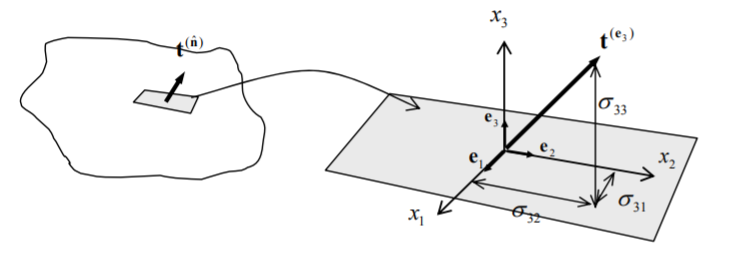
\includegraphics[scale=0.8]{21.png}
	\label{牵引向量的分解:应力分量}
	\caption{text}
\end{figure}
定义牵引矢量$ t $,这个矢量表征了在某参考平面上的一个单元体所受的应力和,即此单元体在此表面处所受的牵引应力。在与 $ e_3 $ 正交的平面上的牵引矢量可以写做
\begin{equation}
\mathbf{t}^{\left(e_{3}\right)}=\sigma_{31} \mathbf{e}_{1}+\sigma_{32} \mathbf{e}_{2}+\sigma_{33} \mathbf{e}_{3}
\end{equation}
其中,$ \sigma_{33} $ 代表此平面上的正应力,以外法线方向为正( 即 $ e_3 $ 正方向 ), $ \sigma_{31} $ 与 $ \sigma_{32} $ 表示平面上的切应力。写出单元体三个面上的牵引向量为:
%\begin{equation}
%\mathbf{t}^{\left(\mathbf{e}_{3}\right)}=t_{1} \mathbf{e}_{1}+t_{2} \mathbf{e}_{2}+t_{3} \mathbf{e}_{3}
%\end{equation}
\begin{equation} \label{eq1}
\begin{aligned} \mathbf{t}^{\left(\mathbf{e}_{1}\right)} &=\sigma_{11} \mathbf{e}_{1}+\sigma_{12} \mathbf{e}_{2}+\sigma_{13} \mathbf{e}_{3} \\ \mathbf{t}^{\left(\mathbf{e}_{2}\right)} &=\sigma_{21} \mathbf{e}_{1}+\sigma_{22} \mathbf{e}_{2}+\sigma_{23} \mathbf{e}_{3} \\ \mathbf{t}^{\left(e_{3}\right)} &=\sigma_{31} \mathbf{e}_{1}+\sigma_{32} \mathbf{e}_{2}+\sigma_{33} \mathbf{e}_{3} \end{aligned}
\end{equation}
式中的 $  \mathbf{e}_{1}~,~ \mathbf{e}_{2} ~,~ \mathbf{e}_{3} $ 的方向如图\ref{fig22}所示。其余各应力的状态也如图\ref{fig2}所示
\begin{figure}
	\centering
	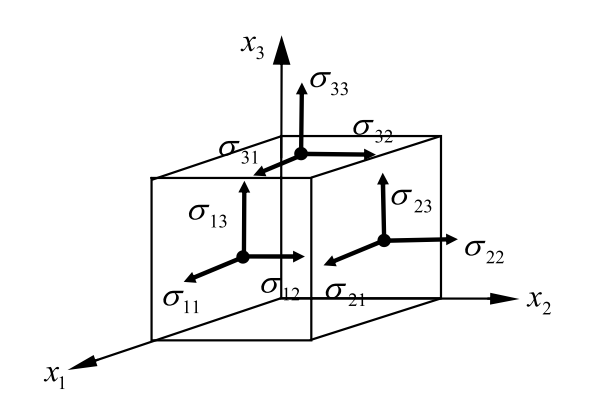
\includegraphics[scale=1.0]{22.png}
	\caption{九个应力分量的状态示意图}
	\label{fig22}
\end{figure}

当然,我们可以使用矩阵来表征这九个分量,图\ref{fig22}状态下的应力矩阵$ [ \sigma_{i j} ] $ 为
\begin{equation}
\left[\sigma_{i j}\right]=\left[ \begin{array}{ccc}{\sigma_{11}} & {\sigma_{12}} & {\sigma_{13}} \\ {\sigma_{21}} & {\sigma_{22}} & {\sigma_{23}} \\ {\sigma_{31}} & {\sigma_{32}} & {\sigma_{33}}\end{array}\right]
\end{equation}

结合\eqref{eq1} 式可得

\begin{equation}
\left[\begin{array}{c}
\mathbf{t}^{\left(\mathbf{e}_{1}\right)} \\
\mathbf{t}^{\left(\mathbf{e}_{2}\right)} \\
\mathbf{t}^{\left(\mathbf{e}_{3}\right)} \\
\end{array}
\right] = 
\left[\sigma_{i j}\right]
\left[
\begin{array}{c}
\mathbf{e}_{1} \\
\mathbf{e}_{2} \\
\mathbf{e}_{3} \\
\end{array}
\right]
 =\left[ \begin{array}{ccc}{\sigma_{11}} & {\sigma_{12}} & {\sigma_{13}} \\ {\sigma_{21}} & {\sigma_{22}} & {\sigma_{23}} \\ {\sigma_{31}} & {\sigma_{32}} & {\sigma_{33}}\end{array}\right]
\left[
\begin{array}{c}
\mathbf{e}_{1} \\
\mathbf{e}_{2} \\
\mathbf{e}_{3} \\
\end{array}
\right]
\end{equation}

在同一单元体上,当选取不同的坐标轴时,相应地导出此坐标轴对应的应力矩阵 $ \left[\sigma_{i j}^{\prime}\right] $ 为:
\begin{equation}
\left[\sigma_{i j}^{\prime}\right]=\left[ \begin{array}{ccc}{\sigma_{11}^{\prime}} & {\sigma_{12}^{\prime}} & {\sigma_{13}^{\prime}} \\ {\sigma_{21}^{\prime}} & {\sigma_{22}^{\prime}} & {\sigma_{23}^{\prime}} \\ {\sigma_{31}^{\prime 1}} & {\sigma_{32}^{\prime \prime}} & {\sigma_{33}^{\prime 3}}\end{array}\right]
\end{equation}

\begin{figure}
	\centering
	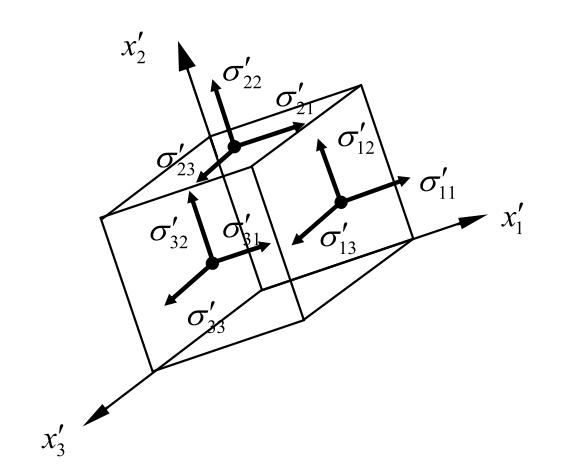
\includegraphics[scale=0.8]{23.png}
	\caption{不同坐标系下九个应力分量的状态示意图}
	\label{fig23}
\end{figure}


\section{柯西定律}

对于更加一般的情况,将上面得到的结论进行推广,即给定了平面和平面上的应力状态,可以根据划分单元体确定平面上的牵引矢量。如图\ref{fig24}所示。$ \textbf{n} $ 代表平面上的法向量,应力状态在图中标明。

\begin{figure}
	\centering
	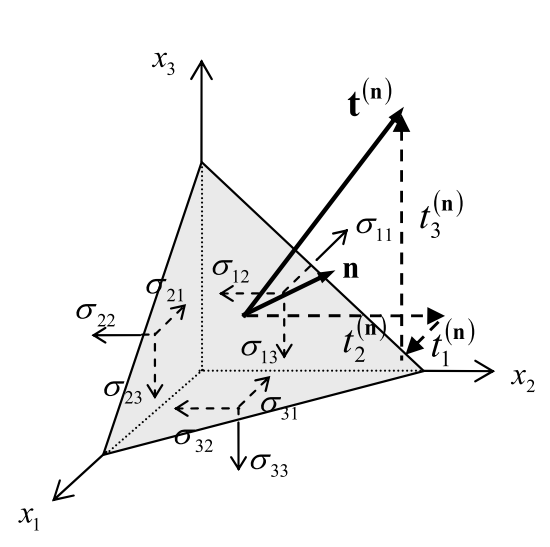
\includegraphics[scale=0.8]{24.png}
	\caption{柯西定律}
	\label{fig24}
\end{figure}

通过上节推导,可得牵引矢量为
\begin{equation}
t_{i}=\sigma_{j i} n_{j}
\end{equation}
将上式写成矩阵形式,牵引矢量、应力分量与平面法向量可写为
\begin{equation}\label{eq2}
\left[t_{i}^{(\mathbf{n})}\right]=\left[ \begin{array}{c}{t_{1}^{(n)}} \\ {t_{2}^{(n)}} \\ {t_{3}^{(n)}}\end{array}\right], \quad\left[\sigma_{i j}\right]=\left[ \begin{array}{ccc}{\sigma_{11}} & {\sigma_{12}} & {\sigma_{13}} \\ {\sigma_{21}} & {\sigma_{22}} & {\sigma_{23}} \\ {\sigma_{31}} & {\sigma_{32}} & {\sigma_{33}}\end{array}\right], \quad\left[n_{i}\right]=\left[ \begin{array}{c}{n_{1}} \\ {n_{2}} \\ {n_{3}}\end{array}\right]
\end{equation}

注意到应力矩阵 $ \left[\sigma_{i j}\right] $ 为\textbf{对称矩阵}。这是因为根据切应力互等定律有如下关系
\begin{equation}
\sigma_{j i} = \sigma_{i j} 
\end{equation}

根据以上推导,可以求出已知应力状态下任意表面的正应力为
\begin{equation}
\sigma_{N}=\mathbf{n} \cdot \mathbf{t}^{(\mathbf{n})}
\end{equation}
其中 $ \mathbf{n} $ 代表表面的法向量。此状态下平面上的剪力为
\begin{equation}
\sigma_{S}=\sqrt{\left|\mathbf{t}^{(\mathbf{n})}\right|^{2}-\sigma_{N}^{2}}
\end{equation}
此平面上的剪力与正应力关系如图\ref{fig25}所示

\begin{figure}
	\centering
	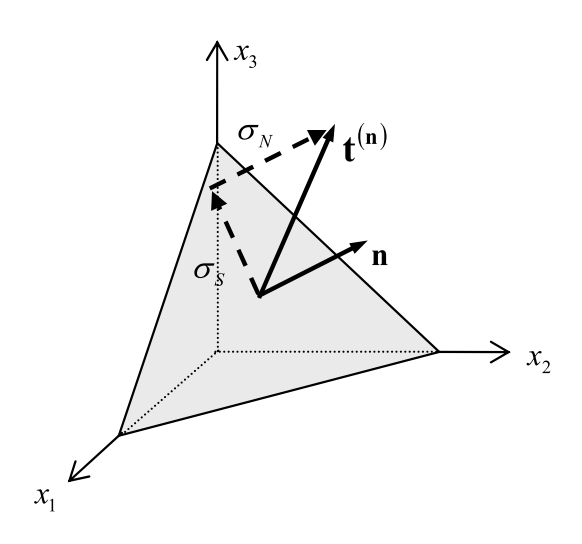
\includegraphics[scale=0.8]{25.png}
	\caption{已知应力状态下任意平面的正应力与切应力}
	\label{fig25}
\end{figure}


\section{转换矩阵}

对于应力状态已知的情况,当考虑从不同方向取单元体,对于其各个截面的应力不尽相同,而此时应力矩阵也不相同。但是不同方向的应力矩阵之间的关系是很容易推导出来的。因为这里将应力矩阵视为一个张量,根据张量变换和线性代数的知识,应力矩阵 $  \left[\sigma_{i j}\right]  $
与 $  \left[\sigma_{i j}^{\prime}\right]  $ 的关系为
\begin{equation}
\left[\sigma_{i j}\right] = \left[Q\right]  \left[\sigma_{i j}^{\prime}\right] \left[Q^T\right]
\end{equation}
式中 $ \left[Q\right]  $ 是一个正交矩阵,此处称为应力转换矩阵。

\begin{figure}
	\centering
	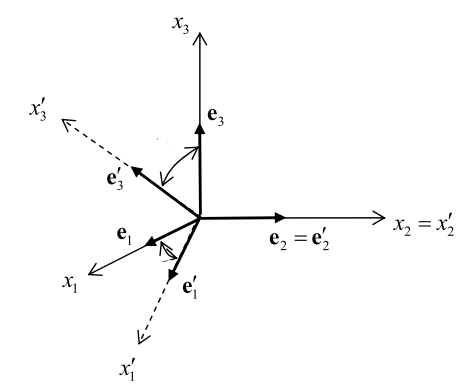
\includegraphics[scale=0.8]{26.png}
	\caption{两个不同坐标系下}
	\label{fig26}
\end{figure}

如\ref{fig26}所示,对于两个不同的右手系坐标轴,写出其应力转换矩阵如下
\begin{equation}
\left[Q_{i j}\right]=\left[ \begin{array}{ccc}{\cos \left(e_{1}, e_{1}^{\prime}\right)} & {\cos \left(e_{1}, e_{2}^{\prime}\right)} & {\cos \left(e_{1}, e_{3}^{\prime}\right)} \\ {\cos \left(e_{2}, e_{1}^{\prime}\right)} & {\cos \left(e_{2}, e_{2}^{\prime}\right)} & {\cos \left(e_{2}, e_{3}^{\prime}\right)} \\ {\cos \left(e_{3}, e_{1}^{\prime}\right)} & {\cos \left(e_{3}, e_{2}^{\prime}\right)} & {\cos \left(e_{3}, e_{3}^{\prime}\right)}\end{array}\right]
\end{equation}
上式中,$ \cos \left(e_{i}, e_{j}^{\prime}\right) $ 代表两个向量之间夹角的余弦。综上,通过借助张量分析中的相关知识,可以实现已知应力状态下任意角度应力矩阵的求解。

\section{主应力的求解}
通过以上的推导,只需要找到特定的应力转换矩阵,就可以很容易的求出主应力。在截面为主平面时,牵引矢量与平面法向量共线,二者成正比,有如下关系
\begin{equation} \label{eq3}
\mathbf{t}=\sigma \mathbf{n}
\end{equation}
式中的 $ \sigma $ 即为主应力。

根据如上关系,可以将\eqref{eq2}带入\eqref{eq3},得到如下关系
\begin{equation}
\mathbf{\sigma} \mathbf{n}=\sigma \mathbf{n}, \quad \sigma_{i j} n_{j}=\sigma n_{i}, \left[ \begin{array}{ccc}{\sigma_{11}} & {\sigma_{12}} & {\sigma_{13}} \\ {\sigma_{21}} & {\sigma_{22}} & {\sigma_{23}} \\ {\sigma_{31}} & {\sigma_{32}} & {\sigma_{33}}\end{array}\right] \left[ \begin{array}{c}{n_{1}} \\ {n_{2}} \\ {n_{3}}\end{array}\right]=\sigma \left[ \begin{array}{l}{n_{1}} \\ {n_{2}} \\ {n_{3}}\end{array}\right]
\end{equation}
将等式化为如下方程
\begin{equation}
(\boldsymbol{\sigma}-\sigma \mathbf{I}) \mathbf{n}=\mathbf{0}
\end{equation}
上式也可以写成如下形式
\begin{equation}
\quad\left(\sigma_{i j}-\sigma \delta_{i j}\right) n_{j}=0
\end{equation}
或
\begin{equation}
\left\{\left[ \begin{array}{ccc}{\sigma_{11}} & {\sigma_{12}} & {\sigma_{13}} \\ {\sigma_{21}} & {\sigma_{22}} & {\sigma_{23}} \\ {\sigma_{31}} & {\sigma_{32}} & {\sigma_{33}}\end{array}\right]-\sigma \left[ \begin{array}{ccc}{1} & {0} & {0} \\ {0} & {1} & {0} \\ {0} & {0} & {1}\end{array}\right]\right\} \left[ \begin{array}{c}{n_{1}} \\ {n_{2}} \\ {n_{3}}\end{array}\right]=\left[ \begin{array}{c}{0} \\ {0} \\ {0}\end{array}\right]
\end{equation}
为了使等式成立,需要左边的矩阵为奇异矩阵,即行列式等于零
\begin{equation}
\left[ \begin{array}{ccc}{\sigma_{11}-\sigma} & {\sigma_{12}} & {\sigma_{13}} \\ {\sigma_{21}} & {\sigma_{22}-\sigma} & {\sigma_{23}} \\ {\sigma_{31}} & {\sigma_{32}} & {\sigma_{33}-\sigma}\end{array}\right] \left[ \begin{array}{l}{n_{1}} \\ {n_{2}} \\ {n_{3}}\end{array}\right]=\left[ \begin{array}{l}{0} \\ {0} \\ {0}\end{array}\right]
\end{equation}
解出 $ \sigma $ 满足如下标量方程,式中
\begin{equation}
\operatorname{det}(\boldsymbol{\sigma}-\sigma \mathbf{I})=\operatorname{det} \left[ \begin{array}{ccc}{\sigma_{11}-\sigma} & {\sigma_{12}} & {\sigma_{13}} \\ {\sigma_{21}} & {\sigma_{22}-\sigma} & {\sigma_{23}} \\ {\sigma_{31}} & {\sigma_{32}} & {\sigma_{33}-\sigma}\end{array}\right]=0
\end{equation}

通过求解以上行列式,能够得到如下的标量方程
\begin{equation}
\sigma^{3}-I_{1} \sigma^{2}+I_{2} \sigma-I_{3}=0
\end{equation}
式中各参量为
\begin{gather}
\begin{array}{c}{I_{1}=\sigma_{11}+\sigma_{22}+\sigma_{33}} \\ {I_{2}=\sigma_{11} \sigma_{22}+\sigma_{22} \sigma_{33}+\sigma_{33} \sigma_{11}-\sigma_{12}^{2}-\sigma_{23}^{2}-\sigma_{31}^{2}} \\ {I_{3}=\sigma_{11} \sigma_{22} \sigma_{33}-\sigma_{11} \sigma_{23}^{2}-\sigma_{22} \sigma_{31}^{2}-\sigma_{33} \sigma_{12}^{2}+2 \sigma_{12} \sigma_{23} \sigma_{31}}\end{array}
\end{gather}
求解此三次方程便可求出任意三向应力状态下的正应力。三次方程的三个根就是三个主应力。显然,这三个主应力是应力矩阵的三个特征值,对应的截面坐标是应力矩阵的特征向量。

\end{document}
